\documentclass[12pt]{report}
\usepackage[utf8]{inputenc}
\usepackage{outline}
\usepackage{amsfonts}
\usepackage{pmgraph}
\usepackage{afterpage}
\usepackage{amsfonts}
\usepackage{amsmath,amssymb,amsthm}
\usepackage{bigstrut}
\usepackage{caption}
\usepackage[english]{babel}
\usepackage{cite}
\usepackage{float}
\usepackage{geometry}
\usepackage{graphicx}
\usepackage{hyperref}
\usepackage[utf8]{inputenc}
\usepackage{listings}
\usepackage{mathtools}
\usepackage{subcaption}
\usepackage{tabularx}
\usepackage{titlesec}
\usepackage{wrapfig}
\usepackage{bm}
\usepackage[normalem]{ulem}
\title{\textbf{Redes Neurais II Primeira Lista de Exercícios}}
\author{Lucas Oliveira David\\ld492@drexel.edu\\l188972}
\date{\oldstylenums{28}/\oldstylenums{09}/\oldstylenums{2016}}

\setlength{\oddsidemargin}{0in}
\setlength{\evensidemargin}{0in}
\setlength{\topmargin}{0in}
\setlength{\headsep}{-.25in}
\setlength{\textwidth}{6.5in}
\setlength{\textheight}{8.5in}

\setlength{\parindent}{1cm}

\begin{document}

\maketitle

\section{Respostas às questões impostas}

\begin{enumerate}
	\item ~\begin{enumerate}
		\item $J(X, \vec y, \theta) = \frac{1}{|X|} \sum_{i = 1}^{|X|}
		        \frac{1}{2}(y_i - sign(a \cdot \vec x_i + b))^2$.

		\item $a= 1.00, b= 1.00, loss = .5$.
		
		\item ~\begin{figure}[H]
			\centering
			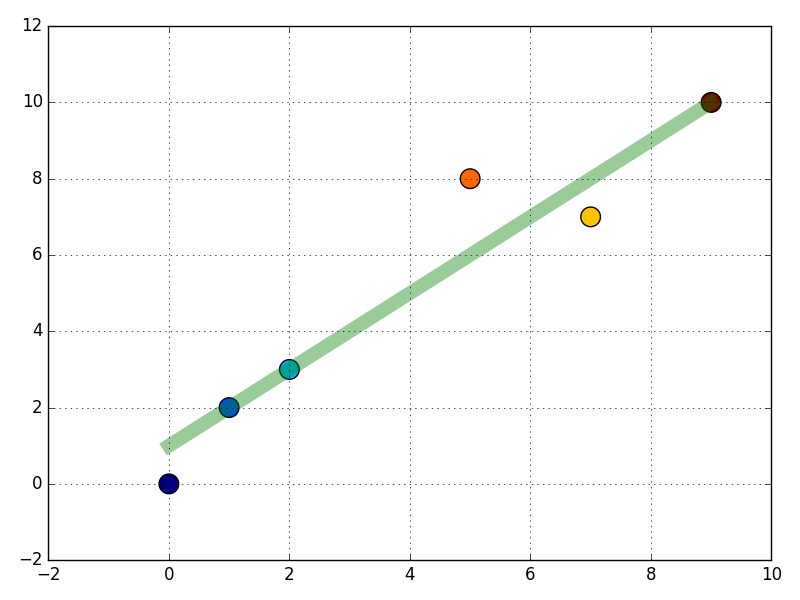
\includegraphics[width=\textwidth]{assets/p1}
			\caption{Desenho da linha de regressão.}
			\label{fig:p1c}
		\end{figure}
	\end{enumerate}
	\item \begin{enumerate}
		\item ~\begin{figure}[H]
			\centering
			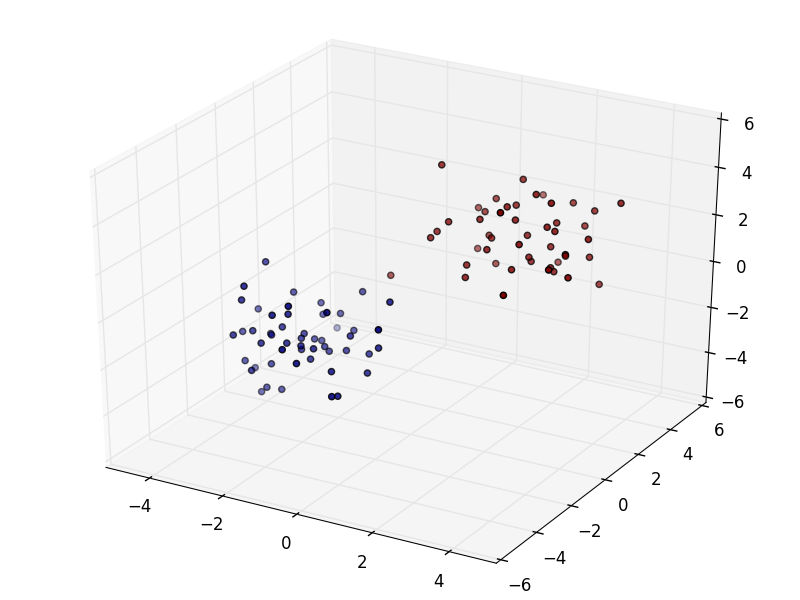
\includegraphics[width=.7\textwidth]{assets/p2}
			\caption{Conjunto de dados 1.}
			\label{fig:p2a}
		\end{figure}
		Aparentam ser linearmente separáveis? Sim.
		
		\item Parâmetros: $\alpha = .1, n\_max\_epochs = 200$.\\
		Resultado: 100\% de acerto, 7 epochs necessários para convergência.\\
		Os padrões são linearmente separáveis: eu achei um hiperplano que
		separa todas as amostras no $\mathbb{R}^3$.
		
		\begin{figure}[H]
			\centering
			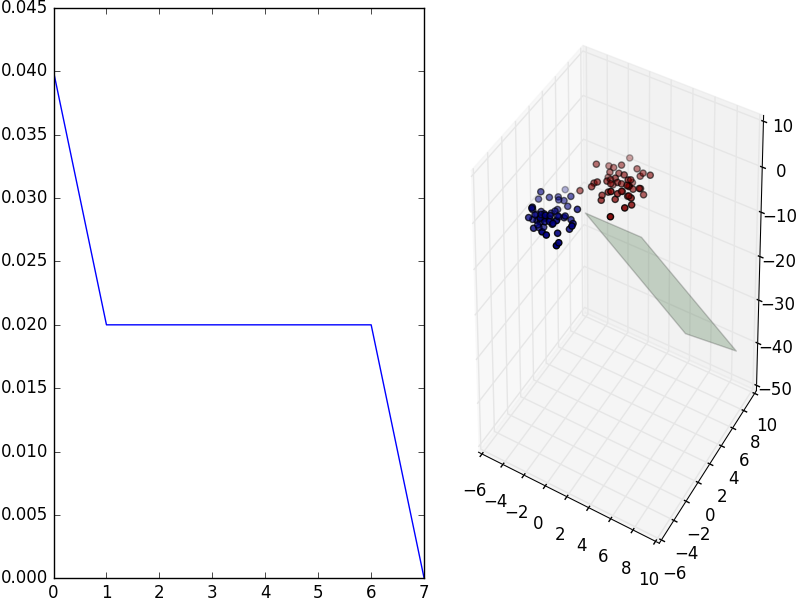
\includegraphics[width=.6\textwidth]{assets/p2b}
			\caption{Conjunto 1 e o hiperplano de separação.}
			\label{fig:p2b}
		\end{figure}
		
		\item Parâmetros: $\alpha = .0001, n\_max\_epochs = 2$.\\
		Resultado: 70\% de acerto.
		
		\begin{figure}[H]
			\centering
			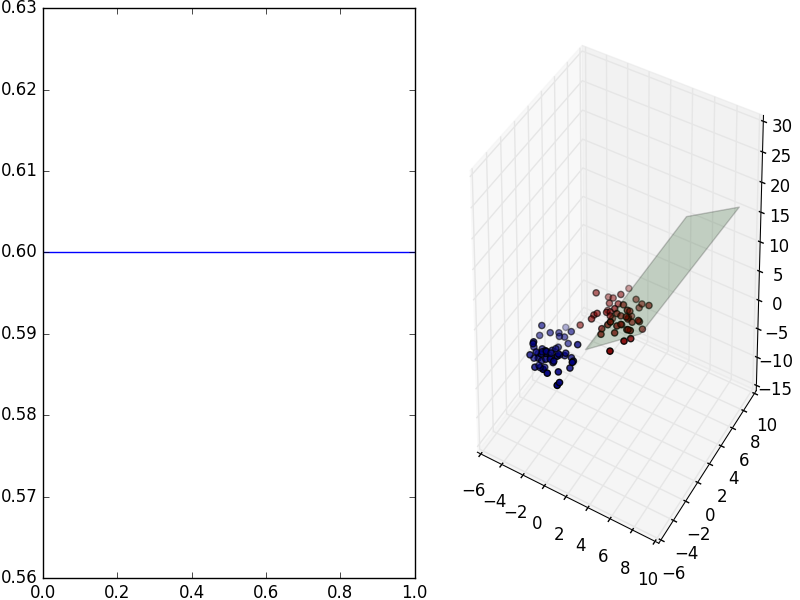
\includegraphics[width=.6\textwidth]{assets/p2c}
			\caption{Conjunto de dados 1 e hiperplano de separação.}
			\label{fig:p2c}
		\end{figure}
		
		\item Parâmetros: $\alpha = .1, n\_max\_epochs = 200$.\\
		Resultado: 100\% de acerto, 13 epochs necessários para convergência.
		
		\begin{figure}[H]
			\centering
			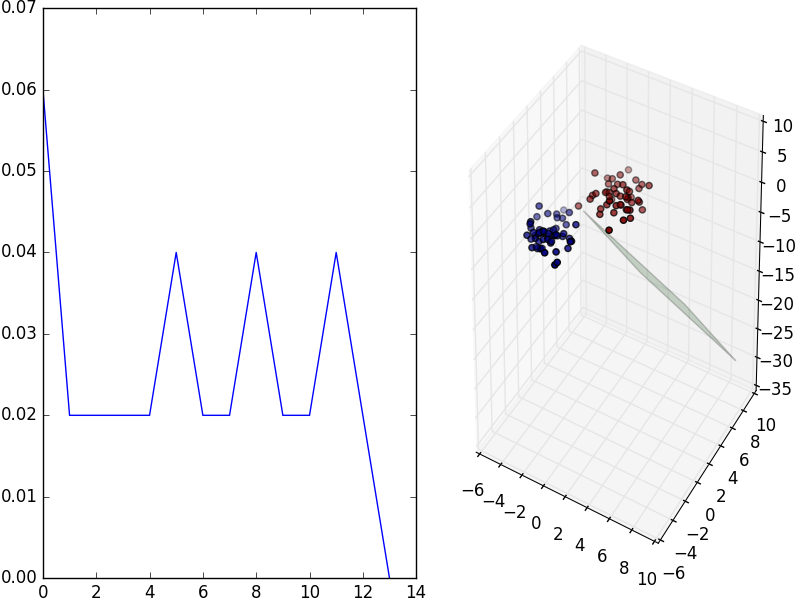
\includegraphics[width=.6\textwidth]{assets/p2d}
			\caption{Conjunto de dados 1 e hiperplano de separação.}
			\label{fig:p2d}
		\end{figure}
	\end{enumerate}
	
	\item ``Grid search" foi empregado para encontrar os melhores parâmetros da
	rede neural. Neste método, cada combinação de parâmetros é utilizada para
	instânciar uma rede diferente. O conjunto de treinamento é separado em 3
	``folds". Duas são utilizadas para treinar o modelo e a última para
	validá-lo. Finalmente, o modelo com maior acurácia é salvo em memória.

	\begin{enumerate}
		\item Parâmetros do \textit{grid}: \{'hidden\_layer\_sizes': [(100,),
		(200,), (1024,)], 'max\_iter': [100, 200, 300]\}.\\
		Melhores parâmetros: \{'max\_iter': 100, 'hidden\_layer\_sizes':
		(100,)\}.\\
		
		Best estimator's score in testing fold: 77\%.\\
		Score on entire dataset: 89\%.\\
		
		Observa-se que o número de unidades e \textit{epochs} que produziu
		melhor resultado sobre o conjunto de validação foram ambos 100, os mais
		baixos. Isso exemplifica o processo de \textit{over-fitting}.

		\item Parâmetros do \textit{grid}: \{'ex\_\_n\_features': [32, 64, 128,
		256, 512, 1024], 'rg\_\_max\_iter': [200],
		'rg\_\_hidden\_layer\_sizes': [(100,), (200,), (1024,), (2048,)]\}
		
		Best parameters: {'ex\_\_n\_features': 32, 'rg\_\_random\_state': 1,
		'rg\_\_hidden\_layer\_sizes': (100,), 'ex\_\_random\_state': 0,
		'rg\_\_max\_iter': 200}.\\
		
		Score on entire dataset: 84\%. Score on entire dataset: 95\%.\\
		
		O melhor resultado obtido foi utilizando uma \textit{extreme machine}
		que projetava as amostras para um espaço de características
		32-dimensional, o mais baixo de todos. Ainda sim, houve um aumento na
		acurácia, em relação à rede treinada em (a).
		
		\item Best estimator found in (a)'s score on dataset 3: 90\%.
		
			  Best estimator found in (b)'s score on dataset 3: 95\%.
			  
			  A pontuação sobre o conjunto de teste (dataset 3) se manteve
			  aproximadamente constante em relação às pontuações obtidas sobre
			  os conjuntos de treinamento e validação. Isso indica que o modelo
			  generalizou adequadamente os padrões contidos no conjunto de
			  treinamento OU que houve \textit{overfitting}, mas que este
			  conjunto de dados contém amostras com baixa variação posicional
			  (pouco ruido).
	\end{enumerate}

	\item O treinamento do modelo de aprendizagem nesta etapa segui os seguintes passos:
	\begin{itemize}
		\item Para cada $c \in \{20, 30, 40, 50, 100\}$:
		\begin{itemize}
			\item O conjunto de dados foi separado em subconjuntos de treinamento (80\%) e
			validação (20\%).
			\item \textit{K-means} foi executado com os parâmetros $\{n\_clusters: c\}$.
			\item Os $c$ centroides encontrados pelo algoritmo $K-means$ foram utilizados
			para iniciar a rede RBF.
			\item A acurácia do modelo treinado sobre o conjunto de treinamento e validação foi computada.
		\end{itemize}
		\item o parâmetro $c$ que induz uma acurácia satisfatória foi escolhido.
		Embora $c=100$ resulte em uma acurácia de 100\%, $c=50$ produz uma de 99\% de maneira
		mais eficiente.
	\end{itemize}
	
	Parâmetros de treino escolhidos: $\{n\_clusters: 50\}$.
	
	Alguns dos 50 centros:
	[ 0.26808911 -0.28454831], [ 1.0557571  -0.92876046], [ 1.16678465  0.95468916], [-0.08038568 -1.10660401], ...
	
	Acurácia no conjunto de treinamento: 99\%\\
	Acurácia no conjunto de validação: 99\%
\end{enumerate}

\end{document}
